\begin{question}{Exercise 7.1}
Answer each part TRUE or FALSE.
\begin{enumerate}[label=\alph*.]
\item $2n=O(n)$.
\item $n^2=O(n)$.
\item $n^2=O(n\log^2 n)$.
\item $n\log n=O(n^2)$.
\item $3^n=2^{O(n)}$.
\item $2^{2^n}=O(2^{2^n})$.
\end{enumerate}
\end{question}
\begin{soln}
Recall Definition~7.2: $f(n)=O(g(n))$ if $c,n_0$ exist with $f(n)\le c\,g(n)$ for all $n\ge n_0$. When $O$ sits in an exponent, $2^{O(n)}$ means $2^{cn}$ for some constant $c$ (p.~278).
\begin{enumerate}[label=\alph*.]
\item TRUE. Take $c=2$: $2n\le 2\cdot n$.
\item FALSE. $n^2/n=n\to\infty$, so no constant $c$ works.
\item FALSE. $n^2/(n\log^2 n)=n/\log^2 n\to\infty$.
\item TRUE. $\log n\le n$ for $n\ge 1$, so $n\log n\le n^2$.
\item TRUE. $3^n=2^{n\log_2 3}$ and $n\log_2 3=O(n)$, so $3^n=2^{O(n)}$.
\item TRUE. Any function is $O$ of itself: take $c=1$.
\end{enumerate}
\end{soln}

\begin{question}{Exercise 7.2}
Answer each part TRUE or FALSE.
\begin{enumerate}[label=\alph*.]
\item $n=o(2n)$.
\item $2n=o(n^2)$.
\item $2^n=o(3^n)$.
\item $1=o(n)$.
\item $n=o(\log n)$.
\item $1=o(1/n)$.
\end{enumerate}
\end{question}
\begin{soln}
Recall Definition~7.5: $f(n)=o(g(n))$ iff $\lim_{n\to\infty}f(n)/g(n)=0$. (In particular $f$ is never $o(f)$, Example~7.6.)
\begin{enumerate}[label=\alph*.]
\item FALSE. $n/(2n)=1/2\not\to 0$.
\item TRUE. $2n/n^2=2/n\to 0$.
\item TRUE. $2^n/3^n=(2/3)^n\to 0$.
\item TRUE. $1/n\to 0$.
\item FALSE. $n/\log n\to\infty$.
\item FALSE. $1/(1/n)=n\to\infty$.
\end{enumerate}
\end{soln}

\begin{question}{Exercise 7.3}
Which of the following pairs of numbers are relatively prime? Show the calculations that led to your conclusions.
\begin{enumerate}[label=\alph*.]
\item $1274$ and $10505$
\item $7289$ and $8029$
\end{enumerate}
\end{question}
\begin{soln}
\textbf{Idea.} Two numbers are relatively prime iff $\gcd=1$ (p.~289). Compute the gcd by the Euclidean algorithm of Theorem~7.15: replace $(x,y)$ by $(y,\,x\bmod y)$ until the remainder is $0$.
\begin{enumerate}[label=\alph*.]
\item
\begin{align*}
10505 &= 8\cdot 1274 + 313,\\
1274 &= 4\cdot 313 + 22,\\
313 &= 14\cdot 22 + 5,\\
22 &= 4\cdot 5 + 2,\\
5 &= 2\cdot 2 + 1,\\
2 &= 2\cdot 1 + 0.
\end{align*}
Thus $\gcd(1274,10505)=1$, so the pair \emph{is} relatively prime.
\item
\begin{align*}
8029 &= 1\cdot 7289 + 740,\\
7289 &= 9\cdot 740 + 629,\\
740 &= 1\cdot 629 + 111,\\
629 &= 5\cdot 111 + 74,\\
111 &= 1\cdot 74 + 37,\\
74 &= 2\cdot 37 + 0.
\end{align*}
Thus $\gcd(7289,8029)=37\neq 1$, so the pair is \emph{not} relatively prime.
\end{enumerate}
\end{soln}

\begin{question}{Exercise 7.4}
Fill out the table described in the polynomial time algorithm for context-free language recognition from Theorem~7.16 for string $w=\mathtt{baba}$ and CFG $G$:
\[
\begin{aligned}
S &\to RT\\
R &\to TR \mid \mathtt{a}\\
T &\to TR \mid \mathtt{b}.
\end{aligned}
\]
\end{question}
\begin{soln}
\textbf{Idea.} $G$ is already in Chomsky normal form, so run algorithm $D$ of Theorem~7.16. The $(i,j)$-entry holds every variable that generates $w_i\cdots w_j$. Fill by increasing substring length, using length-$1$ rules $A\to b$ and then the binary rules $A\to BC$.

Write $w=w_1w_2w_3w_4$ with $w_1=\mathtt{b}$, $w_2=\mathtt{a}$, $w_3=\mathtt{b}$, $w_4=\mathtt{a}$.

\paragraph{Length $1$.}
$table(1,1)=\{\,T\,\}$ because $T\to\mathtt{b}$.
$table(2,2)=\{\,R\,\}$ because $R\to\mathtt{a}$.
$table(3,3)=\{\,T\,\}$ because $T\to\mathtt{b}$.
$table(4,4)=\{\,R\,\}$ because $R\to\mathtt{a}$.

\paragraph{Length $2$.}
Only one split in each substring.
\begin{itemize}
\item $table(1,2)$ (``$\mathtt{ba}$''): $table(1,1)=\{\,T\,\}$ and $table(2,2)=\{\,R\,\}$, so we need a rule $A\to TR$. Both $R\to TR$ and $T\to TR$ apply, hence $\{\,R,T\,\}$.
\item $table(2,3)$ (``$\mathtt{ab}$''): $\{\,R\,\}$ then $\{\,T\,\}$, so $A\to RT$. Only $S\to RT$, hence $\{\,S\,\}$.
\item $table(3,4)$ (``$\mathtt{ba}$''): same as $table(1,2)$, hence $\{\,R,T\,\}$.
\end{itemize}

\paragraph{Length $3$.}
\begin{itemize}
\item $table(1,3)$ (``$\mathtt{bab}$'').
Split $k=1$: $\{\,T\,\}+\{\,S\,\}$ needs $A\to TS$ --- none.
Split $k=2$: $\{\,R,T\,\}+\{\,T\,\}$ needs $A\to RT$ or $A\to TT$. The former is $S\to RT$. So $\{\,S\,\}$.
\item $table(2,4)$ (``$\mathtt{aba}$'').
Split $k=2$: $\{\,R\,\}+\{\,R,T\,\}$ needs $A\to RR$ or $A\to RT$. The latter is $S\to RT$.
Split $k=3$: $\{\,S\,\}+\{\,R\,\}$ needs $A\to SR$ --- none.
So $\{\,S\,\}$.
\end{itemize}

\paragraph{Length $4$.}
$table(1,4)$ (``$\mathtt{baba}$'').
\begin{itemize}
\item Split $k=1$: $\{\,T\,\}+\{\,S\,\}$ needs $A\to TS$ --- none.
\item Split $k=2$: $\{\,R,T\,\}+\{\,R,T\,\}$ needs $A\to RR$, $RT$, $TR$, or $TT$.
$S\to RT$ puts $S$ in the cell; $R\to TR$ puts $R$; $T\to TR$ puts $T$.
\item Split $k=3$: $\{\,S\,\}+\{\,R\,\}$ needs $A\to SR$ --- none.
\end{itemize}
So $table(1,4)=\{\,S,R,T\,\}$. Since $S$ appears there, $D$ accepts: $\mathtt{baba}\in L(G)$.

\begin{center}
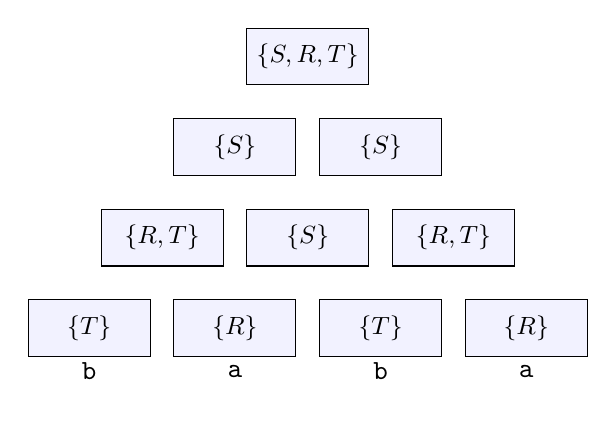
\begin{tikzpicture}[every node/.style={draw,minimum width=1.55cm,minimum height=0.72cm,inner sep=1pt,fill=blue!5,font=\small}]
  \node (a1) at (0,0) {$\{T\}$};
  \node (a2) at (1.85,0) {$\{R\}$};
  \node (a3) at (3.70,0) {$\{T\}$};
  \node (a4) at (5.55,0) {$\{R\}$};
  \node (b1) at (0.925,1.15) {$\{R,T\}$};
  \node (b2) at (2.775,1.15) {$\{S\}$};
  \node (b3) at (4.625,1.15) {$\{R,T\}$};
  \node (c1) at (1.85,2.30) {$\{S\}$};
  \node (c2) at (3.70,2.30) {$\{S\}$};
  \node (d1) at (2.775,3.45) {$\{S,R,T\}$};
  \node[draw=none,fill=none,font=\ttfamily] at (0,-0.55) {b};
  \node[draw=none,fill=none,font=\ttfamily] at (1.85,-0.55) {a};
  \node[draw=none,fill=none,font=\ttfamily] at (3.70,-0.55) {b};
  \node[draw=none,fill=none,font=\ttfamily] at (5.55,-0.55) {a};
\end{tikzpicture}
\end{center}
The pyramid is indexed by substring length (bottom row is length~$1$). Equivalently, as an $n\times n$ table with unused cells below the diagonal:

\begin{center}
\begin{tabular}{@{}c|cccc@{}}
$i\backslash j$ & $1$ & $2$ & $3$ & $4$ \\
\midrule
$1$ & $\{T\}$ & $\{R,T\}$ & $\{S\}$ & $\{S,R,T\}$ \\
$2$ & & $\{R\}$ & $\{S\}$ & $\{S\}$ \\
$3$ & & & $\{T\}$ & $\{R,T\}$ \\
$4$ & & & & $\{R\}$ \\
\end{tabular}
\end{center}
\end{soln}

\begin{question}{Exercise 7.5}
Is the following formula satisfiable?
\[
(x\lor y)\land(x\lor\overline{y})\land(\overline{x}\lor y)\land(\overline{x}\lor\overline{y})
\]
\end{question}
\begin{soln}
\textbf{No.} The four clauses are all possible disjunctions of one literal from $\{x,\overline{x}\}$ and one from $\{y,\overline{y}\}$. Any assignment makes exactly one of $x,\overline{x}$ false and exactly one of $y,\overline{y}$ false, so it falsifies the clause consisting of those two false literals. Explicitly: $xy{=}00$ kills $\overline{x}\lor\overline{y}$; $01$ kills $\overline{x}\lor y$; $10$ kills $x\lor\overline{y}$; $11$ kills $x\lor y$.
\end{soln}

\begin{question}{Exercise 7.6}
Show that $\cP$ is closed under union, concatenation, and complement.
\end{question}
\begin{soln}
\textbf{Idea.} Deciders for $A,B\in\cP$ may be run as subroutines. Union and complement use a constant number of calls; concatenation tries all $O(n)$ split points. Each is polynomial by Definition~7.12 (and Theorem~7.8 if a multitape implementation is more convenient).

Let $M_A$ and $M_B$ decide $A$ and $B$ in time $O(n^k)$ and $O(n^\ell)$ respectively.

\paragraph{Union.}
$M_\cup=$ ``On input $w$:
\begin{enumerate}
\item Run $M_A$ on $w$. If it accepts, \emph{accept}.
\item Run $M_B$ on $w$. If it accepts, \emph{accept}; else \emph{reject}.''
\end{enumerate}
Time $O(n^k)+O(n^\ell)$, hence polynomial. $M_\cup$ accepts iff $w\in A\cup B$.

\paragraph{Concatenation.}
$M_{AB}=$ ``On input $w=w_1\cdots w_n$:
\begin{enumerate}
\item For $i=0$ to $n$:
\item \quad Run $M_A$ on $w_1\cdots w_i$ and $M_B$ on $w_{i+1}\cdots w_n$. If both accept, \emph{accept}.
\item \emph{Reject}.''
\end{enumerate}
There are $n+1$ values of $i$, and each trial uses time $O(n^k)+O(n^\ell)$. Total time $O(n^{1+\max(k,\ell)})$. Correct because $w\in AB$ iff some split has prefix in $A$ and suffix in $B$.

\paragraph{Complement.}
$M_{\mathrm{c}}=$ ``On input $w$: run $M_A$ on $w$; if $M_A$ accepts, \emph{reject}, else \emph{accept}.''
Same running time as $M_A$. $M_A$ is a decider, so this decides $\comp{A}$.
\end{soln}

\begin{question}{Exercise 7.7}
Show that $\NP$ is closed under union and concatenation.
\end{question}
\begin{soln}
\textbf{Idea.} Guess which summand (for union) or which split (for concatenation), then guess the $\NP$-certificates and verify them (Definition~7.19 and Theorem~7.20).

Let $A,B\in\NP$, with polynomial verifiers $V_A,V_B$.

\paragraph{Union.}
Certificate for $w\in A\cup B$: a bit $b\in\{0,1\}$ together with a certificate $c$ for $w$ in $A$ (if $b=0$) or in $B$ (if $b=1$).
Verifier: if $b=0$ run $V_A$ on $\enc{w,c}$; if $b=1$ run $V_B$ on $\enc{w,c}$. Polynomial because $V_A$ and $V_B$ are.

As an NTM: nondeterministically choose to simulate the NTM for $A$ or the NTM for $B$.

\paragraph{Concatenation.}
Certificate for $w=xy\in AB$: the split index $i=|x|$, a certificate $c_A$ that $x\in A$, and a certificate $c_B$ that $y\in B$.
Verifier: check $0\le i\le |w|$, run $V_A$ on $\enc{w_1\cdots w_i,\,c_A}$ and $V_B$ on $\enc{w_{i+1}\cdots w_n,\,c_B}$, and accept if both accept. All of this is polynomial in $|w|$.

As an NTM: nondeterministically cut $w=xy$, then guess and verify the two certificates.
\end{soln}

\begin{question}{Exercise 7.8}
Let $\mathit{CONNECTED}=\{\enc{G}\mid \text{$G$ is a connected undirected graph}\}$. Analyze the algorithm given on page~185 to show that this language is in $\cP$.
\end{question}
\begin{soln}
\textbf{Idea.} The procedure of Example~3.23 (pp.~185--186) is a marking search, the same idea as $\mathit{PATH}\in\cP$ (Theorem~7.14). Each pass marks at least one new node, so the number of passes is at most the number of nodes.

The algorithm is
$M=$ ``On input $\enc{G}$, the encoding of a graph $G$:
\begin{enumerate}
\item Select the first node of $G$ and mark it.
\item Repeat the following stage until no new nodes are marked:
\item \quad For each node in $G$, mark it if it is attached by an edge to a node that is already marked.
\item Scan all the nodes of $G$ to determine whether they all are marked. If they are, \emph{accept}; otherwise, \emph{reject}.''
\end{enumerate}

Let $G$ have $m$ nodes. The input length $n=|\enc{G}|$ satisfies $n=\Omega(m)$.

Stage~1 runs once and is a scan of the node list, time $O(n)$.
Stage~3 runs at most $m$ times: every execution except the last marks a new node, and there are only $m$ nodes. Each execution scans the node list and the edge list, time $O(n)$.
Stage~4 runs once, time $O(n)$.

Total time $O(m\cdot n)=O(n^2)$, which is polynomial. Correctness is the usual one for undirected reachability: a node becomes marked iff it lies in the same component as the first node, so every node is marked iff $G$ is connected. Hence $\mathit{CONNECTED}\in\cP$.
\end{soln}

\begin{question}{Exercise 7.9}
A \emph{triangle} in an undirected graph is a $3$-clique. Show that $\mathit{TRIANGLE}\in\cP$, where $\mathit{TRIANGLE}=\{\enc{G}\mid \text{$G$ contains a triangle}\}$.
\end{question}
\begin{soln}
\textbf{Idea.} The clique size is the constant $3$, so brute-force enumeration of triples is $O(m^3)$ --- polynomial. (Contrast Theorem~7.24 / Corollary~7.43, where the target size $k$ is part of the input and $m^k$ is not a polynomial bound.)

$M=$ ``On input $\enc{G}$, where $G$ is an undirected graph with $m$ nodes:
\begin{enumerate}
\item For every triple of distinct nodes $\{u,v,w\}$:
\item \quad If $\{u,v\}$, $\{v,w\}$, and $\{w,u\}$ are all edges of $G$, \emph{accept}.
\item \emph{Reject}.''
\end{enumerate}

There are $\binom{m}{3}=O(m^3)$ triples. Checking the three edges is a scan of the edge list, time $O(n)$ where $n=|\enc{G}|$. Total time $O(m^3 n)=O(n^4)$. $M$ accepts iff $G$ contains a $3$-clique. Thus $\mathit{TRIANGLE}\in\cP$.
\end{soln}

\begin{question}{Exercise 7.10}
Show that $\mathit{ALL}_{\mathrm{DFA}}$ is in $\cP$.
\end{question}
\begin{soln}
Recall $\mathit{ALL}_{\mathrm{DFA}}=\{\enc{A}\mid \text{$A$ is a DFA and $L(A)=\Sigma^*$}\}$ (Exercise~4.3).

\textbf{Idea.} $L(A)=\Sigma^*$ iff every state reachable from the start state is accepting: a reachable non-accept state is a rejected string, and if every reachable state accepts then every string is accepted. Reachability is the polynomial marking test of Theorem~4.4.

$M=$ ``On input $\enc{A}$, where $A=(Q,\Sigma,\delta,q_0,F)$ is a DFA:
\begin{enumerate}
\item Mark the start state $q_0$.
\item Repeat until no new states are marked:
\item \quad Mark any state that has a transition coming into it from a marked state.
\item If some marked state is not in $F$, \emph{reject}; else \emph{accept}.''
\end{enumerate}

Let $A$ have $s$ states. Stage~3 runs at most $s$ times and each pass inspects every transition, time $O(s\cdot|\Sigma|)$ per pass. Total time $O(s^2|\Sigma|)$, polynomial in $|\enc{A}|$. Hence $\mathit{ALL}_{\mathrm{DFA}}\in\cP$.

(Equivalently: swap accept/non-accept to obtain a DFA for $\comp{L(A)}$, then test emptiness by Theorem~4.4. Complement of a DFA and $E_{\mathrm{DFA}}$ are both polynomial, so this is in $\cP$ as well.)
\end{soln}

\begin{question}{Exercise 7.11}
In both parts, provide an analysis of the time complexity of your algorithm.
\begin{enumerate}[label=\alph*.]
\item Show that $\mathit{EQ}_{\mathrm{DFA}}\in\cP$.
\item Say that a language $A$ is \emph{star-closed} if $A=A^*$. Give a polynomial time algorithm to test whether a DFA recognizes a star-closed language. (Note that $\mathit{EQ}_{\mathrm{NFA}}$ is not known to be in $\cP$.)
\end{enumerate}
\end{question}
\begin{soln}
\paragraph{a.}
\textbf{Idea.} Same construction as Theorem~4.5, but every step is polynomial for DFAs: one product automaton for the symmetric difference, then the emptiness test of Theorem~4.4.

$\mathit{EQ}_{\mathrm{DFA}}=\{\enc{A,B}\mid \text{$A,B$ are DFAs and $L(A)=L(B)$}\}$.
$L(A)=L(B)$ iff the symmetric difference
\[
\bigl(L(A)\cap\comp{L(B)}\bigr)\cup\bigl(\comp{L(A)}\cap L(B)\bigr)
\]
is empty.

$F=$ ``On input $\enc{A,B}$, where $A=(Q_A,\Sigma,\delta_A,q_A,F_A)$ and $B=(Q_B,\Sigma,\delta_B,q_B,F_B)$ are DFAs:
\begin{enumerate}
\item Build the product DFA $C$ with state set $Q_A\times Q_B$ and start $(q_A,q_B)$.
The transition is $\delta_C((p,q),a)=(\delta_A(p,a),\delta_B(q,a))$.
A state $(p,q)$ of $C$ is accepting iff exactly one of $p\in F_A$ and $q\in F_B$ holds.
\item Mark states of $C$ reachable from $(q_A,q_B)$, as in Theorem~4.4.
\item If any marked state is accepting in $C$, \emph{reject}; else \emph{accept}.''
\end{enumerate}

Stage~1 produces $|Q_A|\,|Q_B|$ states, time polynomial in $|\enc{A,B}|$.
Stage~2--3 run in time polynomial in $|C|$, hence in $|\enc{A,B}|$.
$L(C)$ is the symmetric difference, so $L(C)=\emptyset$ iff $L(A)=L(B)$. Thus $\mathit{EQ}_{\mathrm{DFA}}\in\cP$.

\paragraph{b.}
\textbf{Idea.} Always $A\subseteq A^*$. Equality holds iff $\eps\in A$ and $AA\subseteq A$. On a DFA, $\eps\in L(M)$ is ``$q_0$ accepts''. The condition $LL\subseteq L$ means that after reading any string of $L$ (landing in a reachable accept state $p$), every string of $L$ is still accepted from $p$. That is a polynomial number of $\mathit{EQ}_{\mathrm{DFA}}$-style inclusion tests. We must not build an NFA for $L^*$ and call $\mathit{EQ}_{\mathrm{NFA}}$, which is not known to be in $\cP$.

Let $M=(Q,\Sigma,\delta,q_0,F)$ and write $M_p$ for the DFA obtained from $M$ by changing the start state to $p$.

$S=$ ``On input $\enc{M}$, where $M$ is a DFA:
\begin{enumerate}
\item If $q_0\notin F$, \emph{reject}. \quad[[ $\eps\notin L(M)$ ]]
\item Mark every state reachable from $q_0$ (Theorem~4.4).
\item For each reachable accept state $p$:
\item \quad Build the product of $M$ with the complement of $M_p$ (swap $F$ in $M_p$).
\item \quad If that product accepts any string (emptiness test, Theorem~4.4), \emph{reject}.
      \quad[[ some $x\in L(M)$ is rejected from $p$, so $LL\nsubseteq L$ ]]
\item \emph{Accept}.''
\end{enumerate}

\begin{description}
\item[Time.] Stage~2 is polynomial as in~(a). Stage~3 runs $|F|\le|Q|$ times; each product has $|Q|^2$ states and the emptiness test is polynomial in $|Q|$ and $|\Sigma|$. Total polynomial in $|\enc{M}|$.
\item[Correctness.]
If $S$ accepts, then $\eps\in L$ and $L\subseteq L(M_p)$ for every reachable $p\in F$. Thus if $x\in L$ ends in such a $p$ and $y\in L$, the run of $y$ from $p$ accepts, so $xy\in L$. Hence $LL\subseteq L$ and $\eps\in L$, so $L=L^*$.
Conversely, if $L=L^*$ then $q_0\in F$, and for any $x\in L$ ending at a reachable $p\in F$ and any $y\in L$ we have $xy\in L^*=L$, so $y\in L(M_p)$. Thus no product in stage~4--5 accepts, and $S$ accepts.
\end{description}
\end{soln}

\begin{question}{Exercise 7.12}
Call graphs $G$ and $H$ \emph{isomorphic} if the nodes of $G$ may be reordered so that it is identical to $H$. Let $\mathit{ISO}=\{\enc{G,H}\mid \text{$G$ and $H$ are isomorphic graphs}\}$. Show that $\mathit{ISO}\in\NP$.
\end{question}
\begin{soln}
\textbf{Idea.} The reordering itself is a polynomial-length certificate; checking that it preserves edges is a straightforward scan (Definition~7.19, Theorem~7.20).

Certificate: a list $c=(c_1,\dots,c_m)$ of nodes of $H$, intended as the image of the $m$ nodes of $G$ in order.

Verifier $V=$ ``On input $\enc{\enc{G,H},c}$:
\begin{enumerate}
\item Check that $G$ and $H$ have the same number $m$ of nodes and that $c$ is a permutation of the nodes of $H$.
\item For every pair of nodes $u,v$ of $G$, check that $\{u,v\}$ is an edge of $G$ if and only if $\{c(u),c(v)\}$ is an edge of $H$.
\item If both checks pass, \emph{accept}; else \emph{reject}.''
\end{enumerate}

The certificate has length $O(n)$ where $n=|\enc{G,H}|$. Stage~1 is $O(m^2)$ (distinctness). Stage~2 inspects $O(m^2)$ pairs, each by a scan of the edge lists. All polynomial. $G$ and $H$ are isomorphic iff such a permutation exists, so $\mathit{ISO}\in\NP$.

(As an NTM: nondeterministically write a permutation of $V(H)$ and run the same checks.)
\end{soln}

\begin{question}{Problem 7.13}
Let $\mathit{MODEXP}$ be the language of encodings $\enc{a,b,c,p}$ where $a,b,c$, and $p$ are positive binary integers such that $a^b\equiv c\pmod{p}$.
Show that $\mathit{MODEXP}\in\cP$. (Note that the most obvious algorithm doesn't run in polynomial time. Hint: Try it first where $b$ is a power of $2$.)
\end{question}
\begin{soln}
\textbf{Idea.} Multiplying $a$ by itself $b$ times uses $b$ multiplications, and $b$ is exponential in its binary length. If $b=2^k$, then $k$ squarings compute $a^{2^k}$: $a,a^2,a^4,\dots,a^{2^k}$, reducing $\bmod p$ after each step so the integers stay of bit-length $O(|p|)$. General $b$ is a sum of such powers (binary expansion).

$M=$ ``On input $\enc{a,b,c,p}$, positive binary integers:
\begin{enumerate}
\item Set $A\leftarrow a\bmod p$ and $R\leftarrow 1$. Let $b_t\cdots b_0$ be the binary digits of $b$.
\item For $i=0$ to $t$:
\item \quad If $b_i=1$, set $R\leftarrow(R\cdot A)\bmod p$.
\item \quad Set $A\leftarrow(A\cdot A)\bmod p$.
\item If $R\equiv c\pmod{p}$, \emph{accept}; else \emph{reject}.''
\end{enumerate}

\paragraph{Correctness.}
The loop is the standard identity $a^b=\prod_{b_i=1}a^{2^i}$. Reducing $\bmod p$ at each multiplication preserves the residue class, so the final $R$ is $a^b\bmod p$.

\paragraph{Time.}
Let $n=|\enc{a,b,c,p}|$. Then $t<n$ and every intermediate value has $O(n)$ bits. One schoolbook multiplication of $O(n)$-bit numbers is $O(n^2)$; a division for $\bmod p$ is $O(n^2)$. The loop body runs $O(n)$ times, so total time $O(n^3)$. Hence $\mathit{MODEXP}\in\cP$.
\end{soln}

\begin{question}{Problem 7.14}
A \emph{permutation} on the set $\{1,\dots,k\}$ is a one-to-one, onto function on this set. When $p$ is a permutation, $p^t$ means the composition of $p$ with itself $t$ times. Let $\mathit{PERM\text{-}POWER}$ be the language of encodings $\enc{p,q,t}$ where $p$ and $q$ are permutations on $\{1,\dots,k\}$, $t$ is a binary integer, and $p=q^t$.
Show that $\mathit{PERM\text{-}POWER}\in\cP$. (Note that the most obvious algorithm doesn't run within polynomial time. Hint: First try it where $t$ is a power of $2$.)
\end{question}
\begin{soln}
\textbf{Idea.} Same as Problem~7.13, with composition of permutations in place of modular multiplication. Composing $q$ with itself $t$ times is exponential in $|t|$; repeated squaring of permutations is polynomial.

Represent a permutation on $\{1,\dots,k\}$ as the list of $k$ images. Composition $r\circ s$ is the list $\bigl(r(s(1)),\dots,r(s(k))\bigr)$, computable in $O(k)$ array lookups.

$M=$ ``On input $\enc{p,q,t}$:
\begin{enumerate}
\item Check that $p$ and $q$ are permutations of the same set $\{1,\dots,k\}$. If not, \emph{reject}.
\item Set $Q\leftarrow q$ and $R\leftarrow\mathrm{id}$ (the identity permutation). Let $t_\ell\cdots t_0$ be the bits of $t$.
\item For $i=0$ to $\ell$:
\item \quad If $t_i=1$, set $R\leftarrow R\circ Q$.
\item \quad Set $Q\leftarrow Q\circ Q$.
\item If $R=p$ as lists, \emph{accept}; else \emph{reject}.''
\end{enumerate}

\paragraph{Correctness.}
The loop computes $q^t=\prod_{t_i=1}q^{2^i}$ under composition, so $R=q^t$. We accept iff this equals $p$.

\paragraph{Time.}
Let $n=|\enc{p,q,t}|$. Then $k=O(n)$ and $\ell<n$. Each composition is $O(k)=O(n)$, and the loop runs $O(n)$ times, so time $O(n^2)$. Hence $\mathit{PERM\text{-}POWER}\in\cP$.
\end{soln}

\begin{question}{Problem 7.15}
Show that $\cP$ is closed under the star operation. (Hint: Use dynamic programming. On input $y=y_1\cdots y_n$ for $y_i\in\Sigma$, build a table indicating for each $i\le j$ whether the substring $y_i\cdots y_j\in A^*$ for any $A\in\cP$.)
\end{question}
\begin{soln}
\textbf{Idea.} Membership of substrings in $A^*$ obeys the same recurrence as the CFL table of Theorem~7.16: a nonempty string is in $A^*$ iff it is in $A$, or it splits into two nonempty pieces each already known to be in $A^*$. Filling an $n\times n$ table by increasing length uses $O(n^2)$ calls to a decider for $A$.

Let $A\in\cP$ be decided by $M_A$ in time $O(n^k)$. The following decides $A^*$.

$D=$ ``On input $y=y_1\cdots y_n$:
\begin{enumerate}
\item If $n=0$, \emph{accept}. \quad[[ $\eps\in A^*$ always ]]
\item For $1\le i\le j\le n$, initialize $B[i,j]\leftarrow\mathrm{false}$.
\item For $\ell=1$ to $n$: \quad[[ $\ell=$ substring length ]]
\item \quad For $i=1$ to $n-\ell+1$:
\item \qquad Set $j\leftarrow i+\ell-1$.
\item \qquad If $M_A$ accepts $y_i\cdots y_j$, set $B[i,j]\leftarrow\mathrm{true}$.
\item \qquad For $k=i$ to $j-1$:
\item \qquad\quad If $B[i,k]$ and $B[k+1,j]$ are both true, set $B[i,j]\leftarrow\mathrm{true}$.
\item If $B[1,n]$ is true, \emph{accept}; else \emph{reject}.''
\end{enumerate}

\paragraph{Correctness.}
We claim that after the length-$\ell$ pass, $B[i,j]$ is true iff $y_i\cdots y_j\in A^*$. For $\ell=1$ the only possibility is membership in $A$ (stage~6), which is correct. For longer strings: if the substring is in $A$, stage~6 catches it; if it is a concatenation of two nonempty $A^*$ strings, some split is caught in stage~7--8 because shorter cells are already filled. Conversely every nonempty string in $A^*$ is either in $A$ or a concatenation of two nonempty $A^*$ strings. The empty input is accepted in stage~1.

\paragraph{Time.}
There are $O(n^2)$ cells. For each cell we run $M_A$ once, time $O(n^k)$, and inspect $O(n)$ splits. Total $O(n^{k+2}+n^3)$, polynomial. Thus $A^*\in\cP$.
\end{soln}

\begin{question}{Problem 7.16}
Show that $\NP$ is closed under the star operation.
\end{question}
\begin{soln}
\textbf{Idea.} Nondeterministically cut the input into (polynomially many) pieces and guess an $\NP$-certificate for each piece, as in the selected solution.

Let $A\in\NP$. Construct an NTM $N$ that decides $A^*$ in nondeterministic polynomial time.
$N=$ ``On input $w$:
\begin{enumerate}
\item If $w=\eps$, \emph{accept}.
\item Nondeterministically divide $w$ into pieces $w=x_1x_2\cdots x_k$ with each $x_i$ nonempty and $k\le|w|$.
\item For each $x_i$, nondeterministically guess a certificate showing $x_i\in A$.
\item Verify all certificates if possible, then \emph{accept}.
Otherwise, if verification fails, \emph{reject}.''
\end{enumerate}

\paragraph{Correctness.}
$\eps\in A^*$ always. For $w\neq\eps$ we have $w\in A^*$ iff $w=x_1\cdots x_k$ for some $k\ge 1$ and $x_i\in A$; some nondeterministic branch guesses exactly that cut and valid certificates, and stage~4 accepts. If $w\notin A^*$, every cut has some $x_i\notin A$, so every branch fails verification.

\paragraph{Time.}
On a branch, $k\le n:=|w|$ and each certificate has length polynomial in $|x_i|\le n$ (Definition~7.18). Verifying $k$ certificates with a polynomial verifier is polynomial in $n$. By Theorem~7.20, $A^*\in\NP$.
\end{soln}

\begin{question}{Problem 7.17}
Let $\mathit{UNARY\text{-}SSUM}$ be the subset sum problem in which all numbers are represented in unary. Why does the $\NP$-completeness proof for $\mathit{SUBSET\text{-}SUM}$ fail to show $\mathit{UNARY\text{-}SSUM}$ is $\NP$-complete? Show that $\mathit{UNARY\text{-}SSUM}\in\cP$.
\end{question}
\begin{soln}
\textbf{Idea.} The $\NP$-completeness proof for $\mathit{SUBSET\text{-}SUM}$ (Theorem~7.56) writes \emph{short} binary/decimal encodings of \emph{huge} numbers. In unary those same numbers are exponentially long, so the reduction is no longer polynomial. With unary input the target $t$ is at most the input length, and the classical knapsack DP is then polynomial.

Recall
\[
\mathit{SUBSET\text{-}SUM}=\{\enc{S,t}\mid \text{some subcollection of $S$ sums to $t$}\}
\]
(Theorem~7.25; $S$ is a multiset). $\mathit{UNARY\text{-}SSUM}$ is the same language with every integer written in unary.

\paragraph{Why Theorem~7.56 does not carry over.}
The reduction $3\mathrm{SAT}\redp\mathit{SUBSET\text{-}SUM}$ produces, from a formula with $\ell$ variables and $k$ clauses, $O(\ell+k)$ numbers whose decimal representations have $O(\ell+k)$ digits (Figure~7.57). Those numbers have magnitude $10^{\Theta(\ell+k)}$. Writing a number of that magnitude in \emph{unary} takes $10^{\Theta(\ell+k)}$ symbols, which is exponential in $|\enc{\phi}|$. A polynomial-time reduction must output a string of polynomial length, so the same construction is not a polynomial-time reduction to the unary version.

\paragraph{$\mathit{UNARY\text{-}SSUM}\in\cP$.}
Dynamic programming on the target. Let the input be unary numbers $x_1,\dots,x_m$ and unary target $t$. The input length $n$ satisfies $n\ge t+\sum_i x_i$, so $t\le n$ and each $x_i\le n$.

$M=$ ``On input $\enc{x_1,\dots,x_m,t}$ in unary:
\begin{enumerate}
\item Allocate a boolean array $B[0..t]$, set $B[0]\leftarrow\mathrm{true}$ and $B[s]\leftarrow\mathrm{false}$ for $s>0$.
\item For $i=1$ to $m$:
\item \quad For $s=t$ down to $x_i$:
\item \qquad If $B[s-x_i]$ is true, set $B[s]\leftarrow\mathrm{true}$.
\item If $B[t]$ is true, \emph{accept}; else \emph{reject}.''
\end{enumerate}

Invariant: after processing $x_1,\dots,x_i$, the flag $B[s]$ is true iff some subcollection of those $i$ numbers sums to $s$. Scanning $s$ downward prevents using $x_i$ twice in one pass. Time $O(m t)=O(n^2)$. Thus $\mathit{UNARY\text{-}SSUM}\in\cP$.
\end{soln}

\begin{question}{Problem 7.18}
Show that if $\cP=\NP$, then every language $A\in\cP$, except $A=\emptyset$ and $A=\Sigma^*$, is $\NP$-complete.
\end{question}
\begin{soln}
\textbf{Idea.} $\cP\subseteq\NP$ always, so $A\in\NP$. For hardness: $A$ has at least one yes-instance $y_{\mathrm{in}}$ and one no-instance $y_{\mathrm{out}}$; any $B\in\NP$ is in $\cP$ by assumption, so the map that sends members of $B$ to $y_{\mathrm{in}}$ and non-members to $y_{\mathrm{out}}$ is a polynomial-time reduction $B\redp A$ (Definitions~7.29 and~7.34).

Assume $\cP=\NP$ and let $A\in\cP$ with $A\neq\emptyset$ and $A\neq\Sigma^*$.

\paragraph{$A\in\NP$.}
$\cP\subseteq\NP$ holds unconditionally (a polynomial-time decider is a verifier that ignores its certificate). So $A\in\NP$.

\paragraph{Every language in $\NP$ reduces to $A$.}
Fix $y_{\mathrm{in}}\in A$ and $y_{\mathrm{out}}\notin A$ (both exist by the two exclusions). Let $B\in\NP$. Then $B\in\cP$ by hypothesis, so $B$ has a polynomial-time decider $M_B$. Define
\[
f(w)=\begin{cases}
y_{\mathrm{in}}  & \text{if $M_B$ accepts $w$},\\
y_{\mathrm{out}} & \text{if $M_B$ rejects $w$}.
\end{cases}
\]
The map $f$ is polynomial-time computable (run $M_B$, then write a constant string). And $w\in B$ iff $f(w)\in A$, so $B\redp A$.

Therefore $A$ is $\NP$-complete.

\paragraph{Why the two exceptions.}
If $A=\emptyset$, then $f(w)\in A$ never holds, so only $\emptyset$ reduces to $A$. If $A=\Sigma^*$, then $f(w)\in A$ always holds, so only $\Sigma^*$ reduces to $A$. In either case a language such as $\{0\}\in\cP\subseteq\NP$ fails to reduce to $A$, so $A$ is not $\NP$-hard.
\end{soln}
